\documentclass{segabs}
\usepackage{xspace,color,amsmath}
\usepackage{amssymb}
\usepackage{hyperref}
\usepackage{subcaption}
\usepackage{graphicx}
\usepackage{bibentry}
\begin{document}

\title{Inverting for arbitrarily shaped targets using parameterized radial basis functions}

\author{
    Parth Pokar$^1$\& Lindsey J. Heagy$^1$ \\
    $^1$Geophysical Inversion Facility, University of British Columbia \\
}
\email{ppokar@eoas.ubc.ca}

% \footer{Example}
% \lefthead{Pokar \& Heagy}
% \righthead{Parametric RBF inversion}

\maketitle
\begin{abstract}
\vspace{-0.6cm}

We present an inversion technique that provides a robust means for recovering complex, arbitrarily shaped subsurface targets in inversions. By representing the level-set function as a weighted sum of Radial Basis Functions, our approach eliminates the need for a priori assumptions regarding target number or geometry, while significantly reducing the inversion parameter space. Synthetic examples using 2D DC resistivity surveys demonstrate that the method effectively reconstructs complex geological features. Moreover, the framework is inherently adaptable to 3D problems and is applicable to a wide range of geophysical techniques, including magnetics, gravity, electromagnetics, etc., thereby offering a flexible alternative to traditional inversion strategies.
\end{abstract}

\vspace{-0.45cm}
\section{Introduction}
\vspace{-0.25cm}

Inversion of geophysical data is a crucial step in mineral exploration for identifying potential deposits. Mineral deposits are rarely simple; they often exhibit curvy, irregular, and non-smooth geometries. Accurately representing these complex shapes is particularly important prior to drilling, but remains a challenge for conventional inversion techniques.

Traditional least squares regularized inversion techniques struggle with shapes that have sharp edges or small physical property contrasts. An alternative is parametric shape-based inversion, where shapes such as rectangular prisms \citep{belliveau_parametric_2023} or ellipsoids \citep{mcmillan_3d_2015} are deformed using a set of associated parameters to recover the target. Parametric methods offer the significant advantage of reducing the total parameter space of the inverse problem. These methods, however, have notable drawbacks: (1) they require prior knowledge and initialization of the expected number of targets; (2) they perform poorly if the target deviates from the assumed parameterized shape.

Methods based on parametric basis functions have been shown to be able to address these issues  \citep{aghasi_parametric_2011,kadu_salt_2017, ozsar_parametric_2025}. Instead of selecting a predefined parameterized shape, approaches based on Radial Basis Functions (RBFs) offer the benefits of parametric inversion without imposing strict shape constraints.

In this work, we adapt the RBF method originally described by \citep{aghasi_parametric_2011}. We parameterize the model space with a user-defined number of RBFs, each associated with scalar weights that serve as the inversion parameters. The RBFs form a level-set function that is binarized using a chosen indicator function, which defines the width of the boundary between the shape and background model helping to delineate the target shape. The level-set is updated during the inversion to find a model that fits the data. We validate this method using two models. The first features two distinct targets: a rectangular block and a sphere, while the second contains an anomaly with an arbitrary shape. Both are imaged using a 2D DC Resistivity (DCR) survey. The anomaly is treated as a level-set with fixed conductivity. While we demonstrate the method in 2D DCR, it is not limited to this setting. The approach is both method- and dimension-agnostic and has been successfully applied to 3D problems and other geophysical data types, including potential field and seismic data \citep{kadu_salt_2017}.

\vspace{-0.45cm}
\section{Level-Set Approach to Inversion}
\vspace{-0.25cm}

In geophysical inverse problems, a common goal is to determine the location, shape, and physical properties of a target of interest in a heterogeneous background. Consider a general inverse problem where the forward model is:
\begin{equation}
	F(\mathbf{m}) + \eta = \mathbf{d}
\end{equation}
with $\mathbf{m}$ representing the discretized model, $\mathbf{d}$ the observed data, and $F$ the forward operator that maps the model to the data space. Here, $\eta$ is the noise in the data, usually assumed to be Gaussian.

For level-set methods, we define the shape and location of the target as the $c$ level-set of some function ${\phi(\mathbf{x})} = c$ where $\mathbf{x}$ denotes the spatial coordinates in model space and $c$ is a scalar (usually taken to be zero). In cases where one or more anomalous bodies in present in a background, the overall model space can then be discretized as
 \begin{equation}\label{model_eq}
\mathbf{m(x, p)} = \mathbf{m_0(x)} + H\big(\mathbf{\phi(x,p)}\big)\mathbf{m_p(x)}
\end{equation}
where $\mathbf{m_0(x)}$ is the background model and $\mathbf{m_p(x)}$ describes the physical properties of the anomalous bodies; in the simplest case, $\mathbf{m_0(x)}$ and and $\mathbf{m_p(x)}$ are scalars. Here, $\mathbf{m_p}$ is multiplied by a level-set function $\phi(\mathbf{x},\mathbf{p})$, where $\mathbf{p}$ is a vector of parameters determined during inversion. The level-set is refined by an indicator function, $H$, which defines the boundary of the level-set domain $\Omega$ (and hence the boundary of the target). A general form of the indicator function is a step function:
$$H(\mathbf{x}) = \begin{cases}
	1, & \text{for } \mathbf{x} \ \in \  \Omega\\
	0, & \text{otherwise}
\end{cases}$$

For parametric level-set methods, the level-set function $\phi(\mathbf{x})$ is represented in terms of a set of parameters $\mathbf{p}$. In geometric parameterizations (e.g., ellipses or prisms), $\mathbf{p}$ might include the location of the shape’s centre, strike and dip extents, rotation angles, etc. \citep{belliveau_parametric_2023}. In contrast, this work eschews geometric parameterization of the level-set function in favour of Radial Basis Functions (RBFs), given that any smooth level-set function can be approximated by a linear combination of a set of sufficiently smooth RBFs \citep{aghasi_parametric_2011}.

We first define a set of RBFs, $\psi(\mathbf{r})$, centred on a grid with a spacing ($\mathbf{x_{rbf}}$) that is sparser than the simulation grid (denoted by $\mathbf{x}$). Here, $\mathbf{r} = \mathbf{x} - \mathbf{x_{rbf}}$. Then, we represent the level-set function as a weighted sum of these RBFs:
\begin{equation}\label{rbf_param}
\phi(\mathbf{x},\mathbf{p}) = \sum_{j=1}^{n_{rbf}} \alpha_j  \psi\Big(\beta \| \mathbf{x} - \mathbf{x}_{rbf,j}\|\Big)\end{equation}
where $\alpha_j$ is the scaling parameter for the $j^{th}$ RBF, and $\beta$ is the dilation parameter that determines its width (Figure \ref{fig:rbf}).

There are various choices of RBF, such as Gaussian, thin-plate splines, multiquadratic, compactly-supported RBFs, etc. In shape-reconstruction inverse problems, Gaussian and Wendland functions are commonly used. In this study, we employ the $C^6$ Wendland function as it is shown to improve the sparsity of the system matrices, reduce the computational cost, and recover sharper edges\citep{aghasi_parametric_2011}. The $C^6$ Wendland function is defined as \begin{equation}\label{wendland}
\psi(\mathbf{r})  = (1 - r)^8_+ (32r^3 + 25r^2 + 8 r + 1)
\end{equation} where $(1-r)_+$ denotes that the term is non-zero only when $r<1$.

\begin{figure}[h]
    \centering
    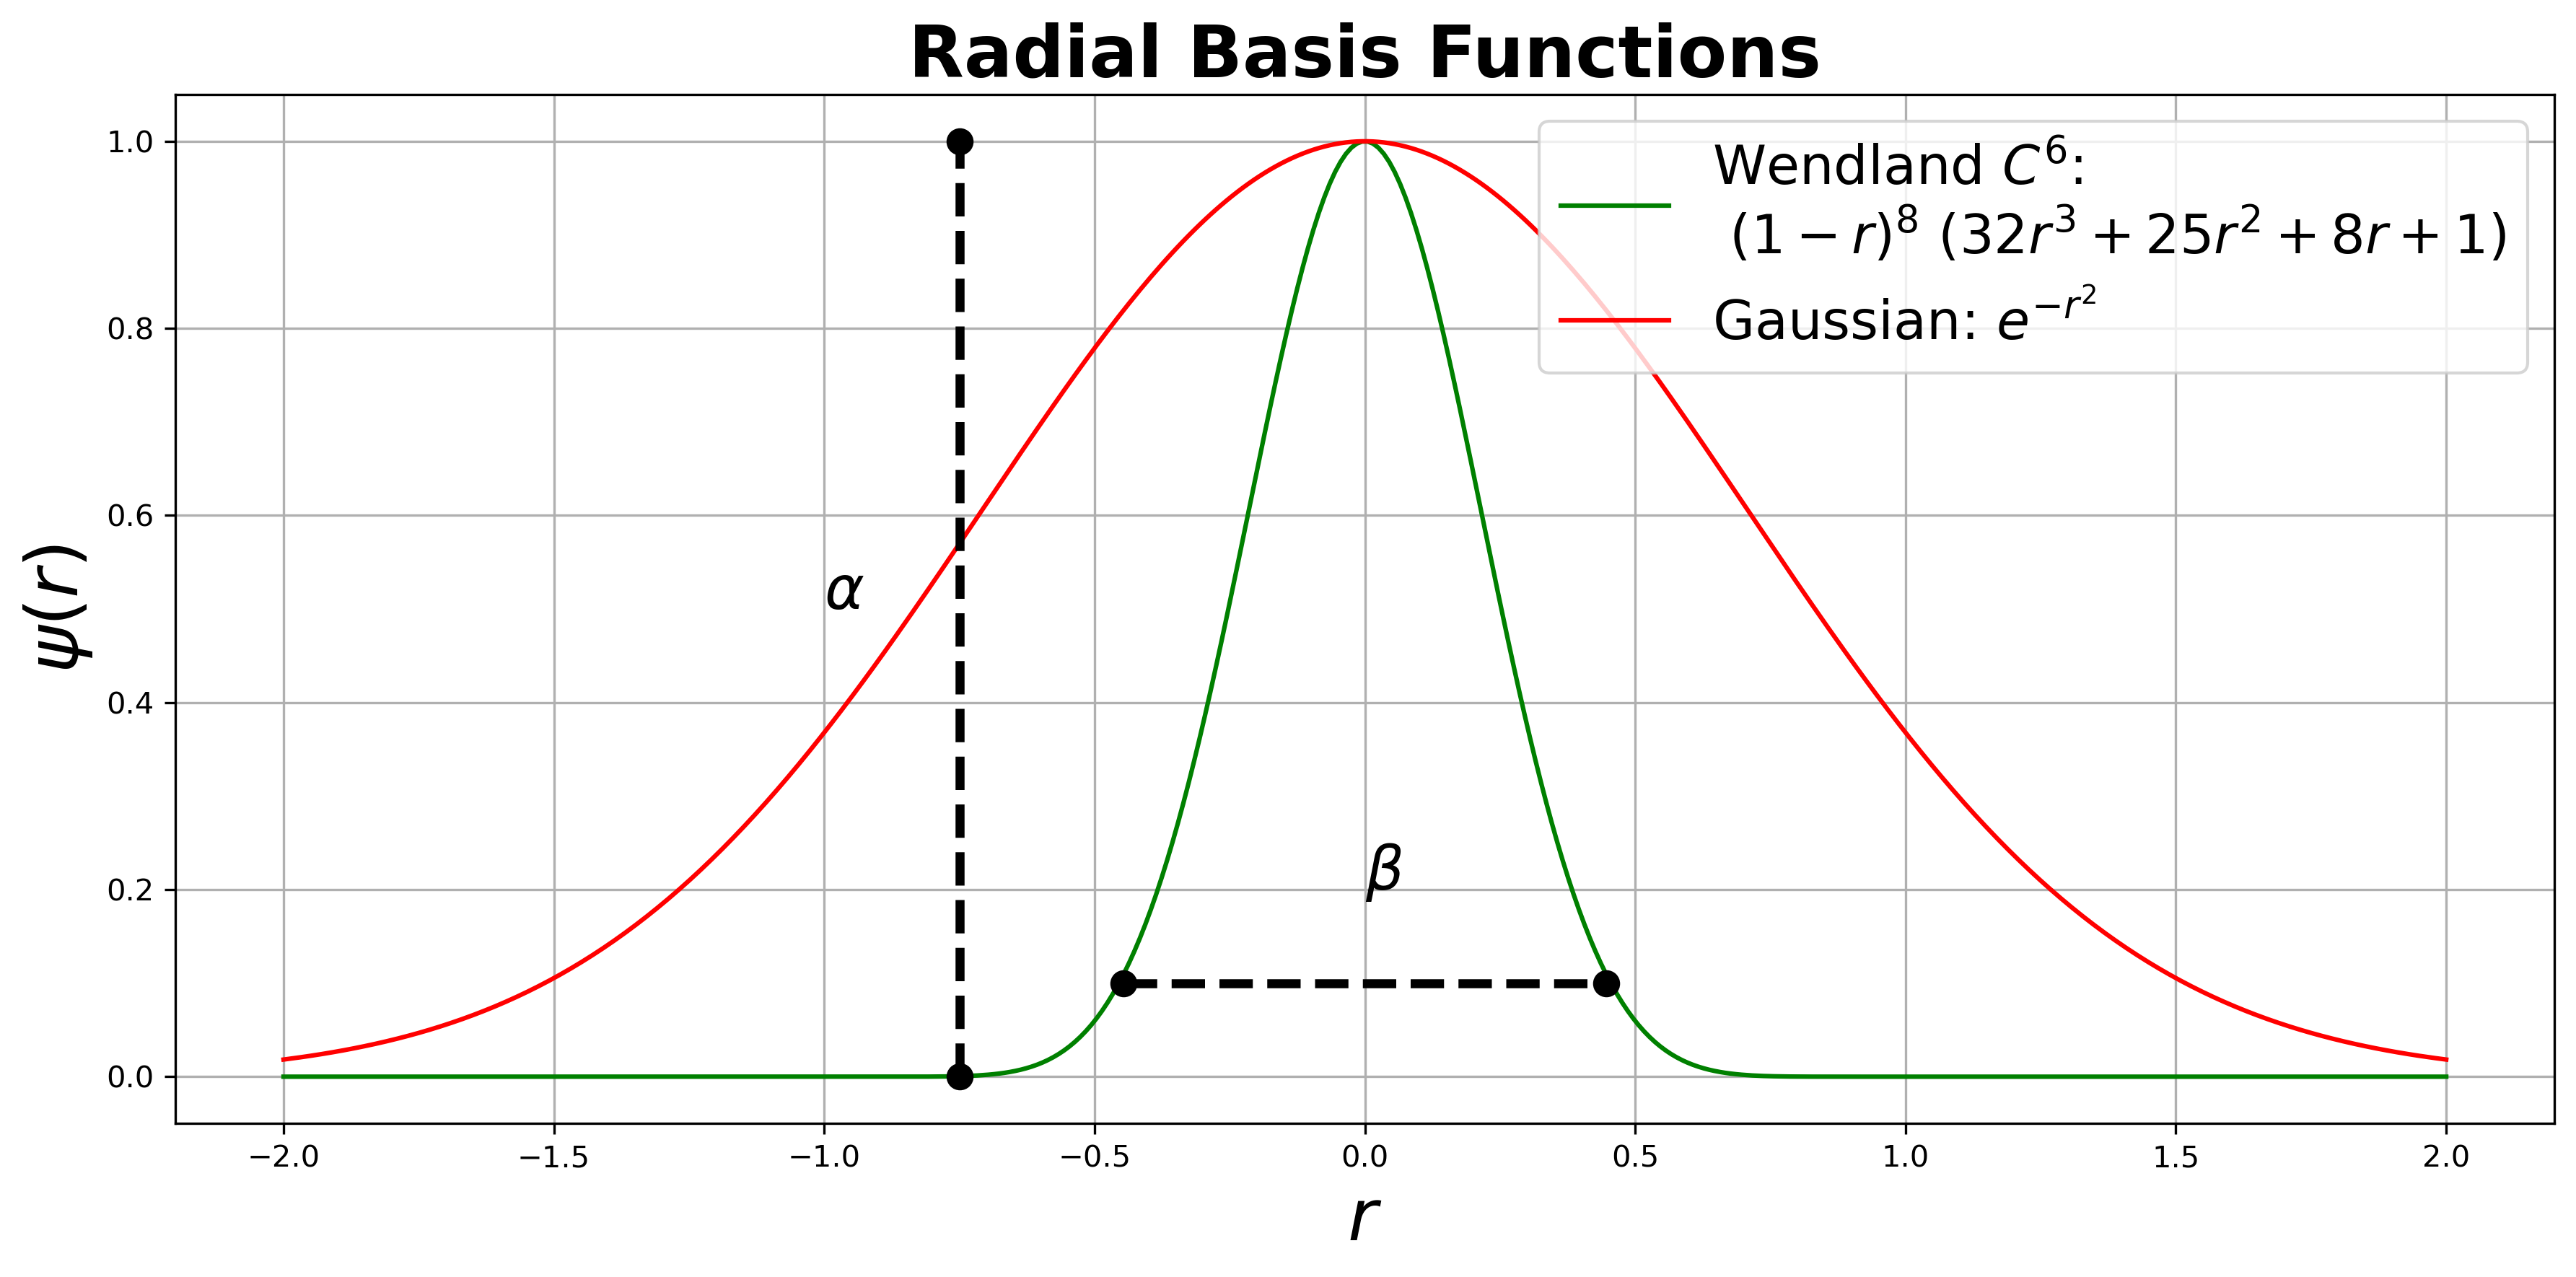
\includegraphics[width=\columnwidth]{figures/rbf_func.png}
    \caption{Comparison between Gaussian and Wendland radial basis functions. The compactness of Wendland RBF (green) relative to Gaussian (red) RBF is useful in recreating sharper features in the shape.}
    \label{fig:rbf}
\end{figure}
In general, one can choose to parameterize the level-set function with $\mathbf{p} = [\boldsymbol{\alpha}, \beta, \mathbf{x}_{rbf}]$. For even greater flexibility, further parameters (such as stretching or skewing of each basis) can be introduced \citep{ozsar_parametric_2025}.  However, in this study, we only treat $\boldsymbol{\alpha}$ as the inversion parameters, keeping $\beta$ and $\mathbf{x}_{rbf}$ fixed. This choice reduces the dimensionality and improves numerical stability, since multiple pairs of $[\alpha, \beta]$ can yield the same $\phi(\mathbf{x}, \mathbf{p})$. A positive value of $\alpha_j$ produces a positive “bump” in the level-set function, with higher values increasing the sharpness—thus aiding in resolving sharp corners or edges of a target.

We fix the dilation parameter as $\beta = 1/\Delta_{rbf}$, where $\Delta_{rbf}$ is the spacing between RBF centers (typically between 2 and 4 times the simulation mesh spacing). The RBF centers $\mathbf{x}_{rbf}$ are defined on an equally spaced grid and remain fixed during the inversion.

Another choice is the selection of the Heaviside function. Since an ideal Heaviside function (a step function) is non-differentiable, a smooth sigmoid approximation is preferred. A common choice is a sigmoid function. We use a regularized ${C^2}$ Heaviside function following \cite{aghasi_parametric_2011}:
\begin{equation}\label{heavyside}
H\big[\phi(\mathbf{x},\epsilon)\big] = \begin{cases}
	1, & \phi<\epsilon \\
	0, & \phi>-\epsilon\\
        \frac{1}{2} + \frac{\phi}{2\epsilon}+ \frac{1}{2\pi}\sin(\frac{\pi \phi}{\epsilon}), & |\phi| \leq \epsilon
\end{cases}
\end{equation}

\begin{figure}[h]
    \centering
    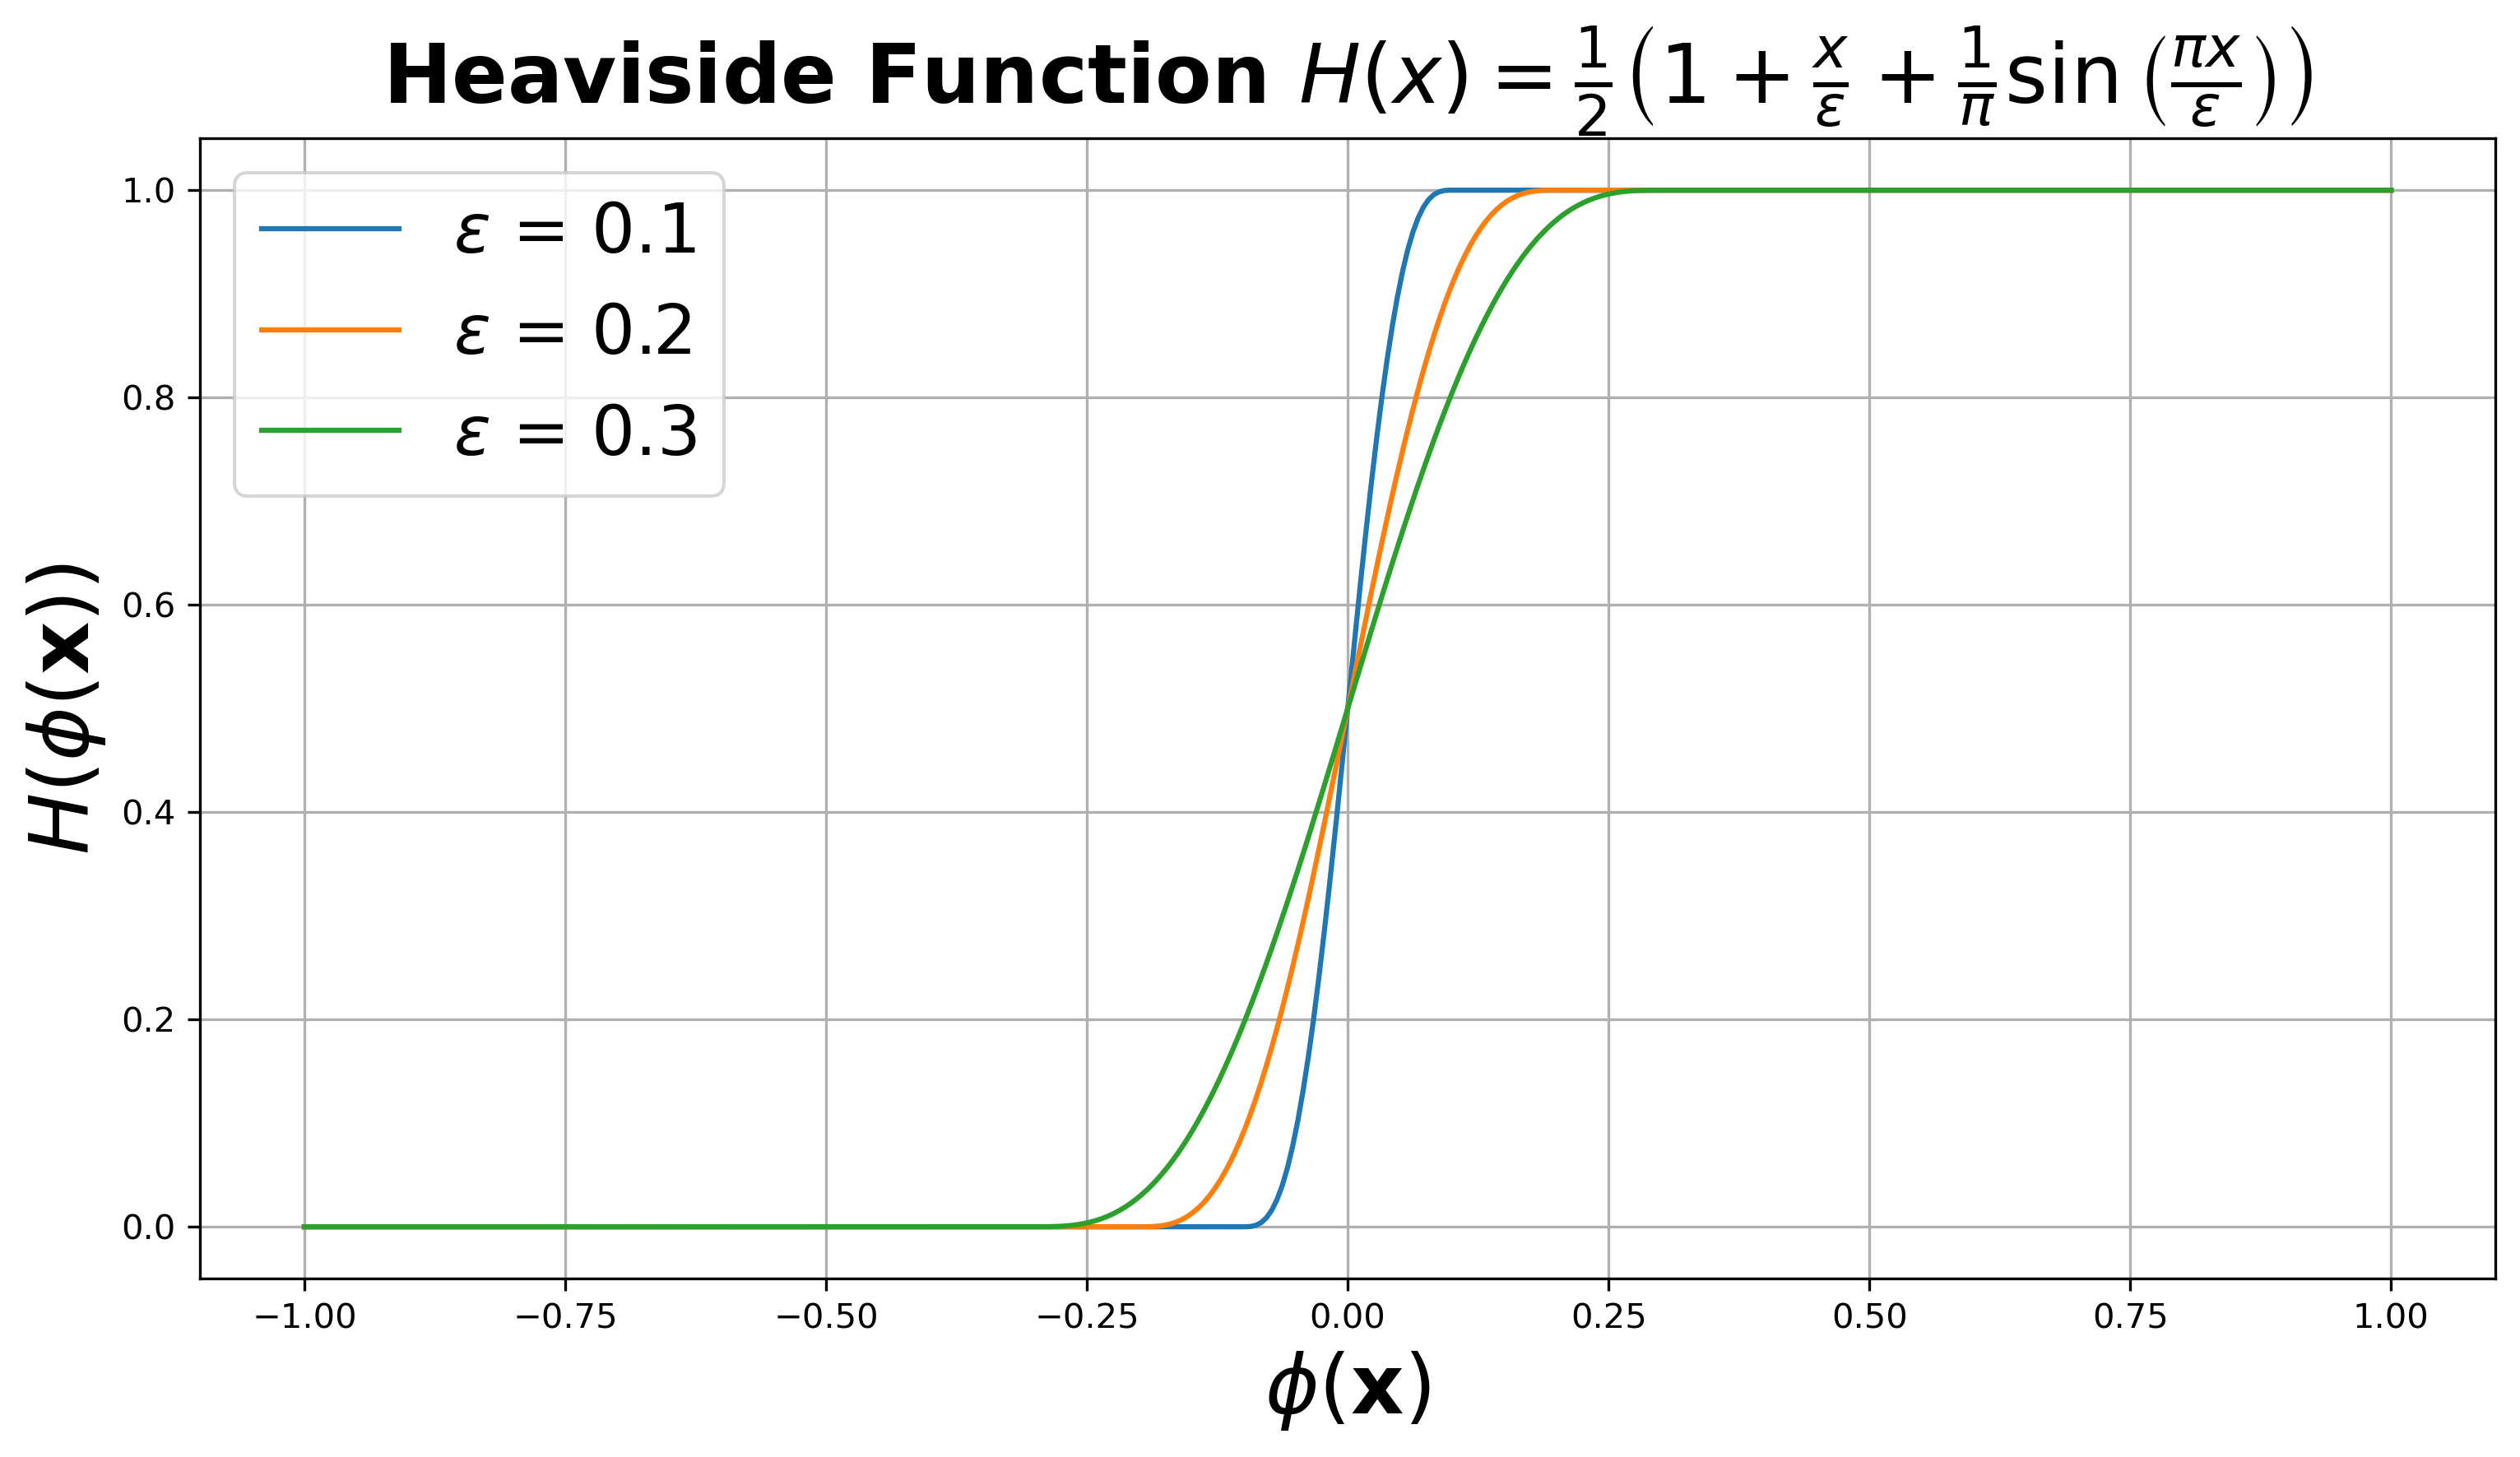
\includegraphics[width=\columnwidth]{figures/heaviside.png}
    \caption{Heaviside function (eq \ref{heavyside}) used to binarize the level set function $\phi(\mathbf{x}, \mathbf{p})$. Higher $\epsilon$ increases the transition region of the level set, improving numerical stability but reducing resolution}
    \label{fig:heaviside}
\end{figure}

Figure \ref{fig:heaviside} illustrates this Heaviside function. Here, $\epsilon$ controls the steepness of the transition; choosing an appropriate $\epsilon$ is crucial, as an overly steep or flat transition can lead to numerical instabilities (e.g., vanishing gradients).

We update $\epsilon$ at each iteration and define it as a fraction of the dynamic range of the level-set function \citep{kadu_salt_2017}:
\begin{equation}\label{trans_width}
\epsilon = \gamma\big(\phi_{max} - \phi_{min}\big)
\end{equation}

We include $\gamma$ as an additional inversion parameter.

Thus, the inverse problem is formulated as a minimization of a misfit function with respect to the inversion parameters $\mathbf{p} = [\boldsymbol{\alpha}, \gamma]$:

\begin{equation}\label{inv_prob}
\min_{\mathbf{p}} ||F\big(\mathbf{m(x,p)}\big) - \mathbf{d}|| + \lambda R({\mathbf{p}})
\end{equation}
where $\lambda$ is a weighting factor for the regularization term $R$ that can be applied to the parameters $\mathbf{p}$.

We then invert the data by solving the minimization problem in equation \eqref{inv_prob} using a Gauss-Newton optimization method. The necessary derivatives are computed automatically via the \textit{autograd} functionality in PyTorch \citep{ansel_pytorch_2024}.

\vspace{-0.45cm}
\section{Examples}
\vspace{-0.25cm}

We test our inversion approach using a synthetic 2D DC resistivity survey. Two model scenarios are examined: one containing compact targets (a block and a circular target) in a halfspace, and one where we aim to estimate depth to a basement layer. The data are generated for a dipole-dipole configuration with electrodes spaced every 50 m along $x = [-1000, 1000]$ on a flat topography. All simulations and inversions are performed using the SimPEG package \citep{heagy_framework_2017,cockett_simpeg_2015}.

\subsection{Example 1: Multiple Compact Targets}
\vspace{-0.4cm}

We consider the model shown in Figure \ref{fig:block_sphere}a consisting of a 400 m $\times$ 200 m rectangular block centred at [250, -200], and a circular target with a 150 m radius centred at [-600, -200] in a homogeneous halfspace. This model is chosen to evaluate the method's ability to resolve multiple targets with different geometries. The simulation mesh uses a 40 $\times$ 40 cell grid with 50 m spacing, resulting in 800 active cells.

First, we show an inverted model that is recovered using a regularized weighted least-squares method, starting from a halfspace model (Figure \ref{fig:block_sphere}b). The inverted model is able to image the targets in approximately the correct locations but the boundaries of the shapes are smooth and difficult to interpret. For the parametric RBF inversion, we initialize the model (Figure \ref{fig:block_sphere}c) with 187 RBFs distributed uniformly every 150 m within the active region of the mesh. The $\mathbf{\alpha}$ parameters are drawn from a normal distribution with a standard deviation of 0.1. To reduce the influence of RBFs located below the survey's sensitivity (below $z = -500$ m), these are assigned a large negative weight ($\alpha = -10$) to dampen their impact on the inversion. No explicit regularization is enforced (i.e., $\lambda=0$ in equation \eqref{inv_prob}) in the parametric RBF inversion, making this step necessary to prevent overfitting. We initialize the $\gamma$ parameter in equation \ref{trans_width} as 0.1, corresponding to 10\% of the dynamic range of the initial level-set function. The conductivity values for the background and targets, $m_0$ and $m_p$ respectively, are set to match those of the true model. Absent a-priori information, the physical properties can also be included as additional parameters in the inversion.

Our inverted model (Figure \ref{fig:block_sphere}d) successfully recovers the geometry of both targets. The inversion forms a parametric level-set function whose zero-level set delineates two distinct, compact targets. This result highlights the advantage of our approach: it can recover multiple shapes without prior information, unlike other parametric methods that require the number of targets to be specified at initialization.

\begin{figure}[b]
    \centering
    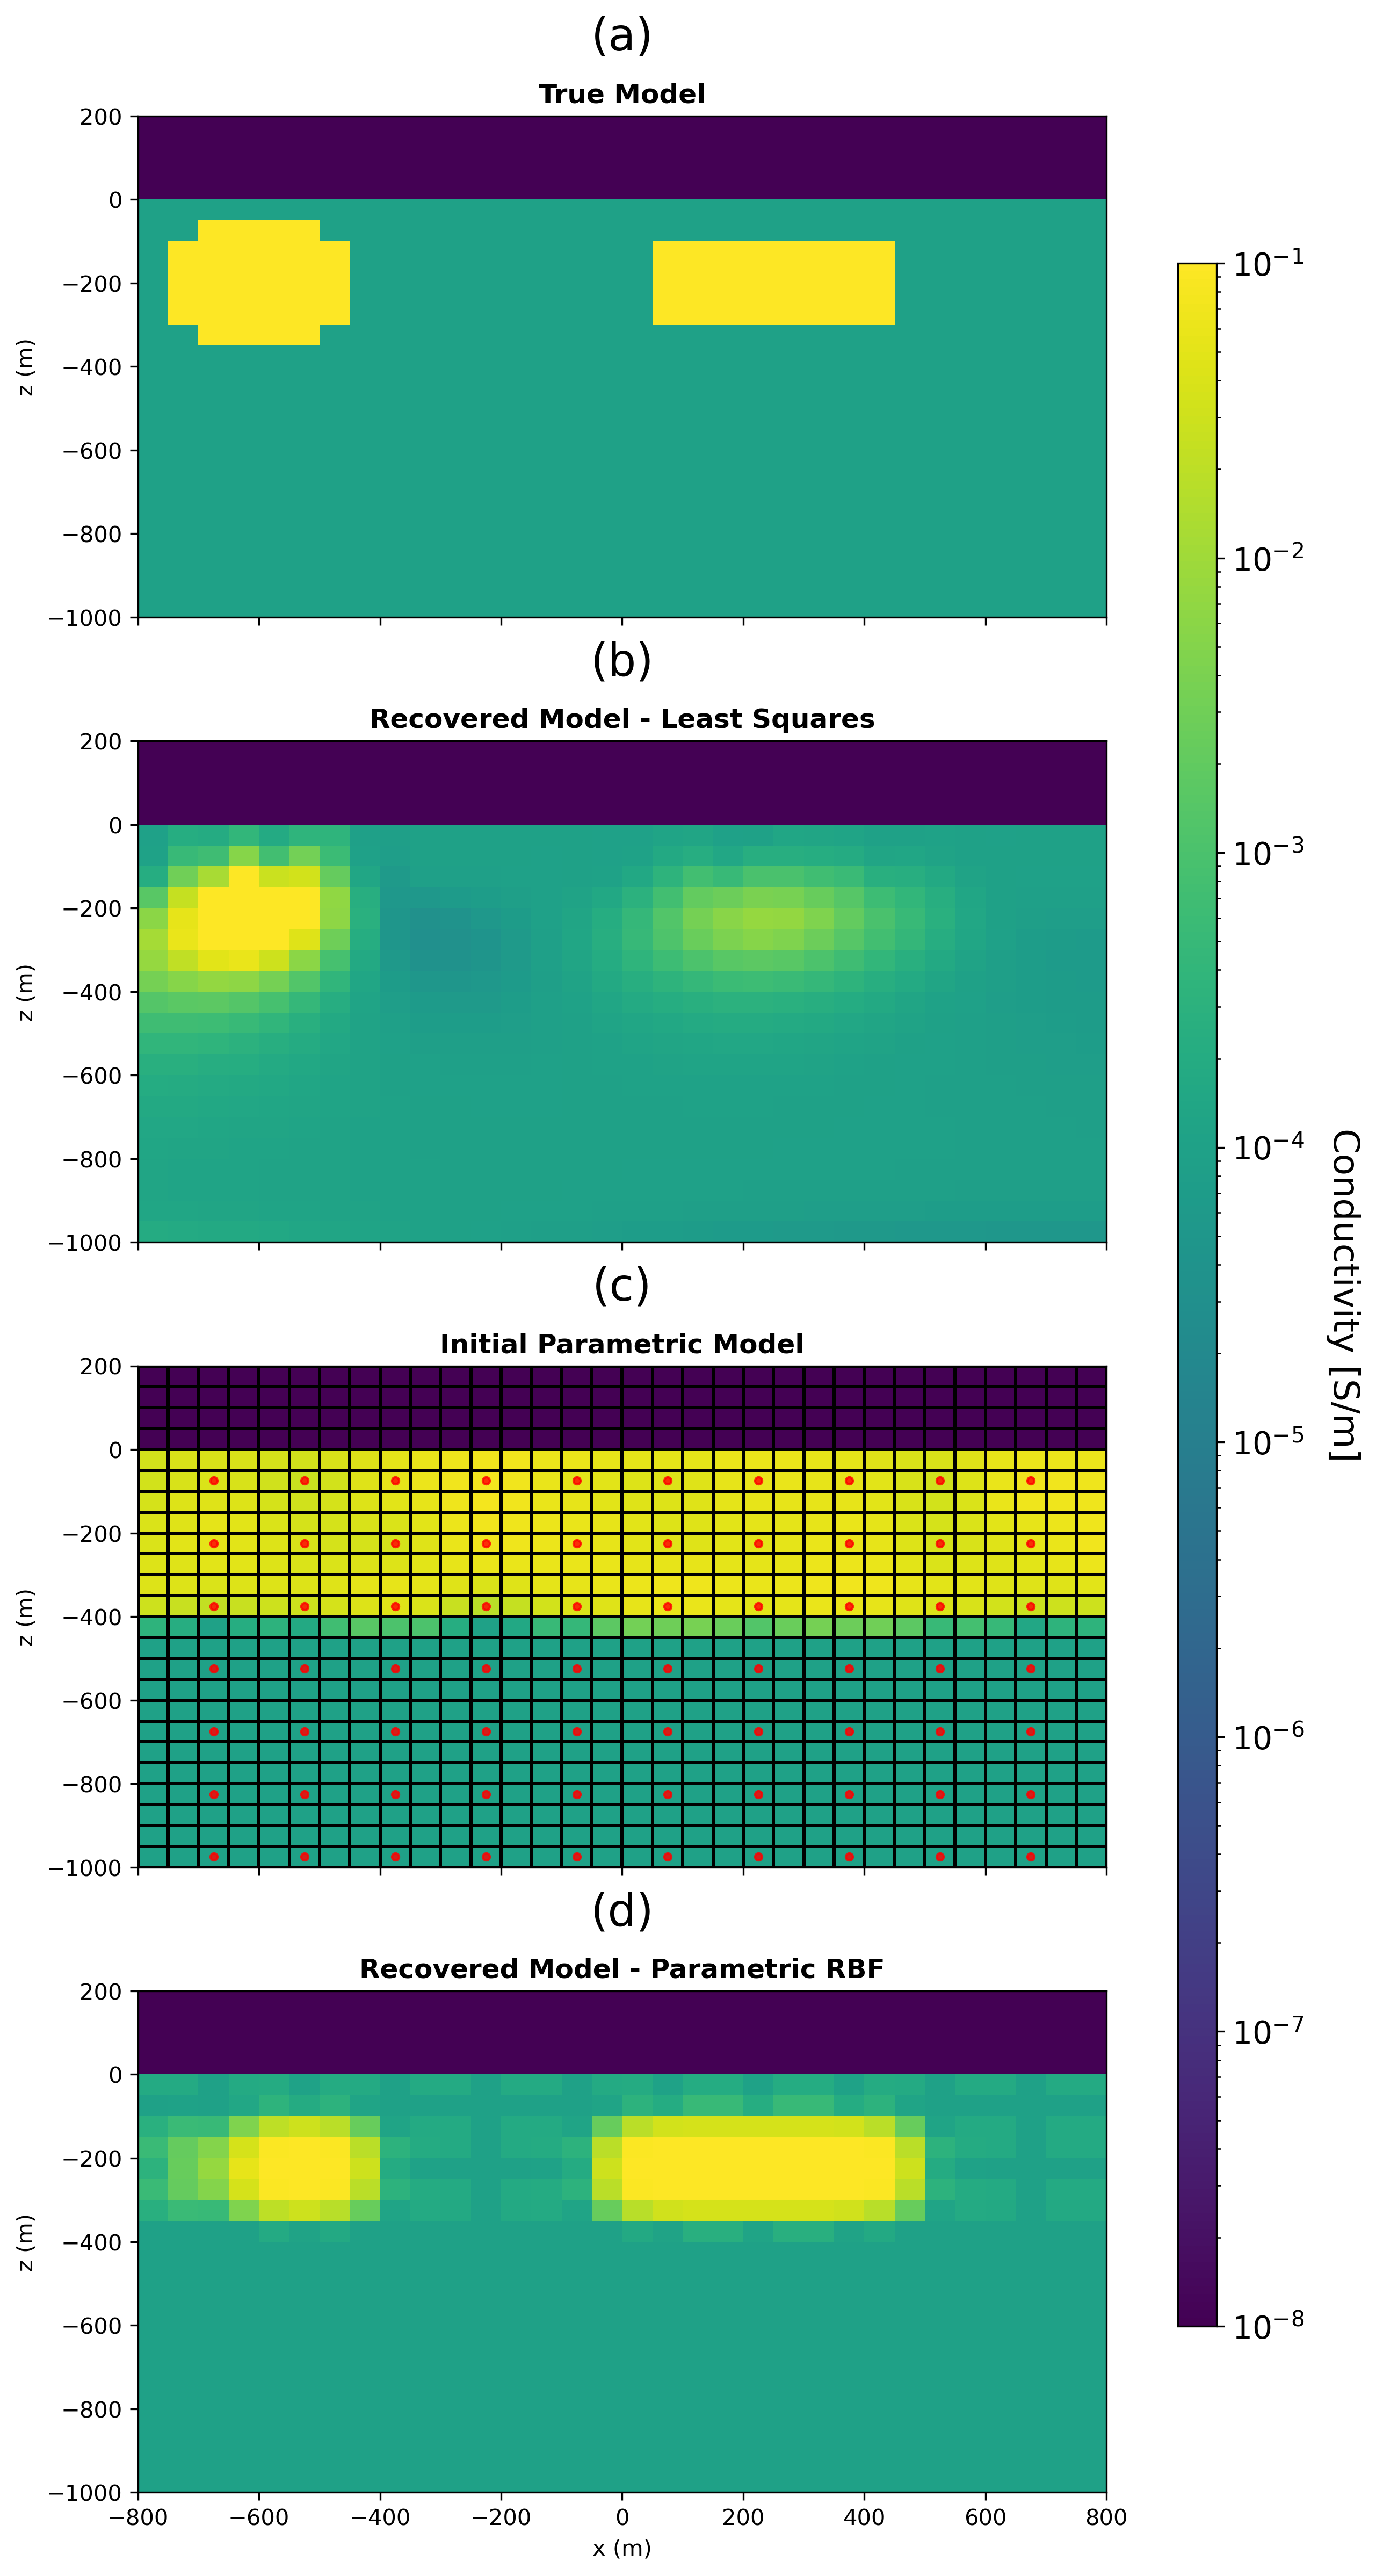
\includegraphics[width=\columnwidth]{figures/block_all_4_title.png}
    \caption{ \textbf{(a)} True model for a synthetic example with a rectangular block and circular targets in a halfspace imaged using a 2D DCR survey. \textbf{(b)} Inverted model using regularized weighted least-squares approach. \textbf{(c)} Initial model for the parametric RBF approach showing the simulation grid (black) and RBF grid (red). Note the sparsity of the RBF grid. \textbf{(d)} Inverted model using the parametric RBF approach without explicit regularization. }
    \label{fig:block_sphere}
\end{figure}

\subsection{Example 2: Depth to Basement}
\vspace{-0.4cm}

To further evaluate our method, we test it on a model that simulates depth-to-basement variations. The true model (Figure \ref{fig:d2b}a) represents a two-layer Earth with a higher-conductivity lower layer (the \lq\lq basement\rq\rq) whose depth varies sinusoidally. At its shallowest the basement is at $z=-200$ m and further along the line the basement deepens up to $z=-500$ m. The simulation mesh uses a 40 $\times$ 40 cell grid with 50 m spacing, resulting in 800 active cells.

For the RBF inversion (Figure \ref{fig:d2b}b), the RBFs are arranged similarly to the previous example but are spaced every 200 m, resulting in 128 parameters to be estimated in the inversion. The $\alpha$ parameters are again initialized from a normal distribution with a standard deviation of 0.1. Here, RBFs located above $z = -600$ m are assigned a large negative weight ($\alpha = -10$) to introduce a conductive layer in the initial model at a depth where the survey starts losing sensitivity. This constraint is necessary in the absence of explicit regularization.

The resulting inverted model (Figure \ref{fig:d2b}c) effectively recovers the undulating structure of the basement layer, despite the limited sensitivity of the survey at these depths.

\begin{figure}[h]
    \centering
    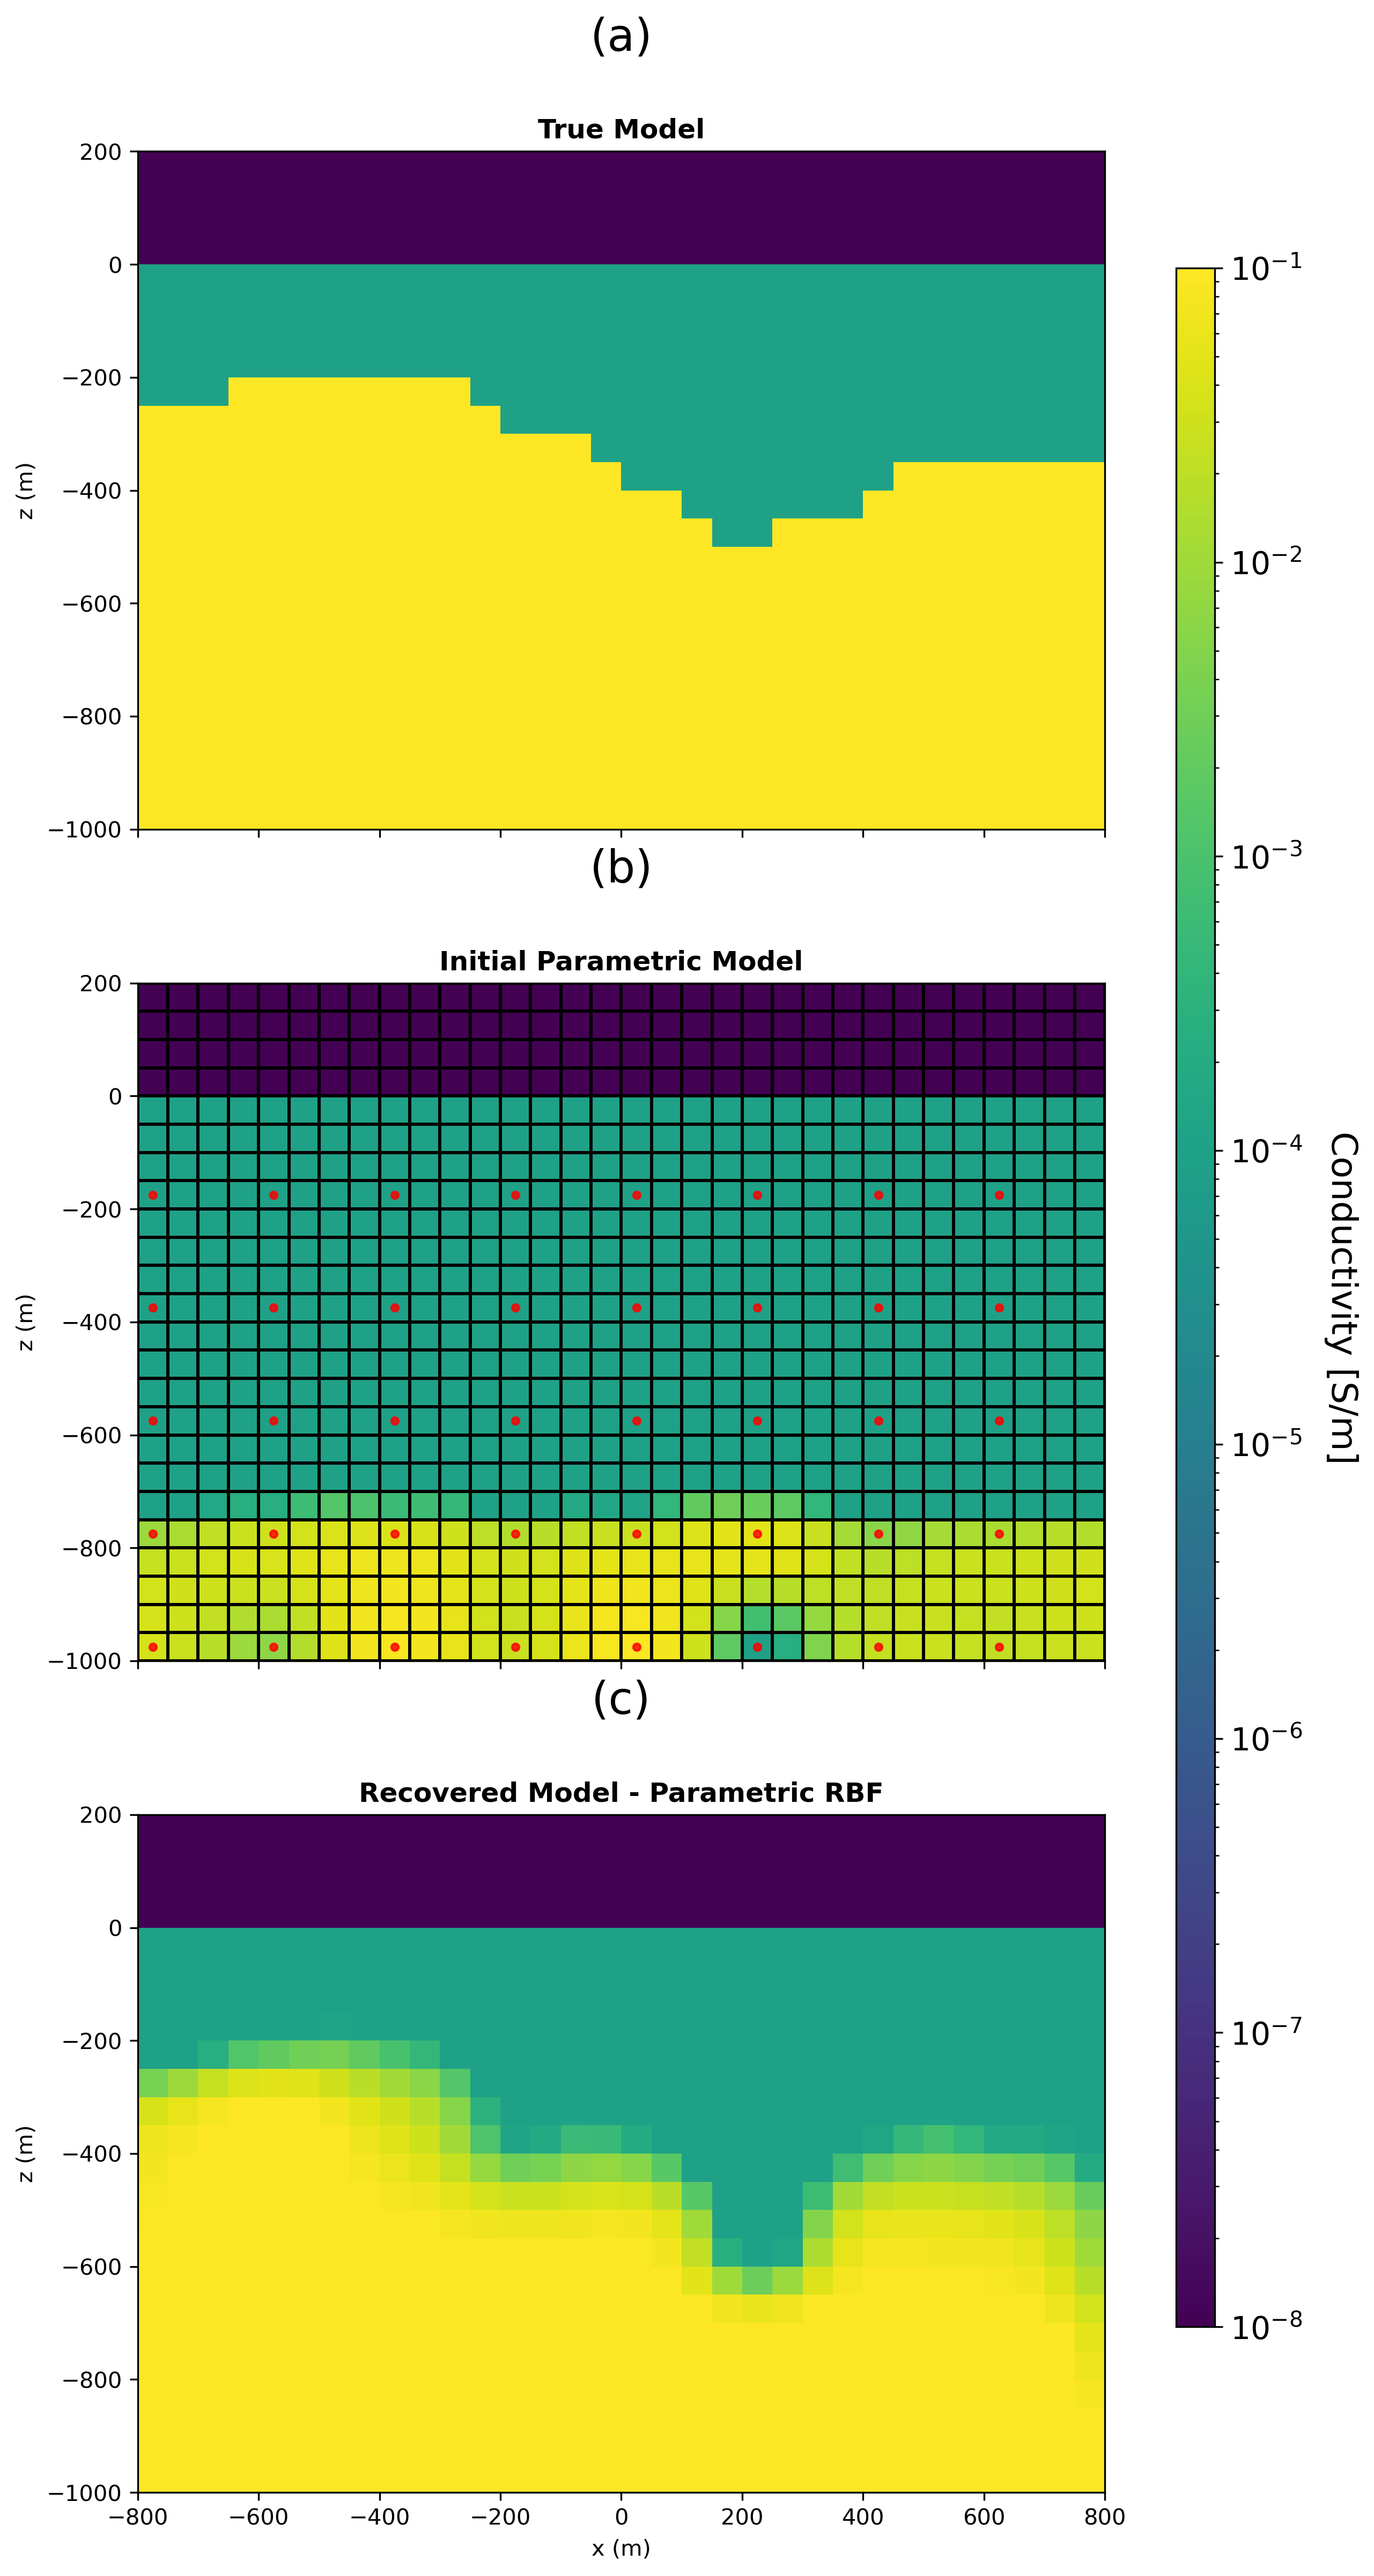
\includegraphics[width=\columnwidth]{figures/d2b_all_3_title_v2.png}
    \caption{ \textbf{(a)} True model for a synthetic example of a two-layer earth with an undulating basement layer. \textbf{(b)} Initial model for the parametric RBF approach showing the simulation grid (black) and RBF grid (red). \textbf{(c)} Inverted model for the depth-to-basement scenario using the parametric RBF approach without explicit regularization.}
    \label{fig:d2b}
\end{figure}

\vspace{-0.45cm}
\section{Conclusion}
\vspace{-0.25cm}

In this work, we have demonstrated that the RBF level-set approach offers a flexible framework for geophysical inversion. Our results highlight the method’s ability to recover arbitrarily shaped features, as illustrated by both the compact targets in a halfspace and the undulating basement in a two-layer model. Importantly, the approach does not require a priori knowledge of the number or geometry of targets, setting it apart from traditional parametric methods.

While our examples focused on 2D DC resistivity surveys, the method is inherently generalizable and can be applied to 3D problems as well as other geophysical techniques, including magnetics, gravity, electromagnetic, and seismic methods.

Our future work will focus on combining this method with hybrid inversion techniques where a weighted least squares inversion can be used to estimate any heterogeneity in the background physical properties \citep{belliveau_parametric_2023}. This information can be incorporated into the model parameterization ($\mathbf{m_0}$ term in equation \ref{model_eq}) or as a reference model for regularization. Another focus will be designing appropriate regularization in the RBF parametric model space. Early efforts show that adding regularization is helpful in introducing a priori knowledge, particularly outside the core sensitivity region of the surveys.

The inversion process still requires careful selection of bounds and an appropriate initial model to ensure numerical stability. In our experience, the RBF approach is more robust to the initial model as compared to geometric parameterization approaches. Additionally, resolving multiple bodies with different physical properties remains challenging without specialized modifications. Our ongoing research focuses on addressing this limitation by incorporating anisotropic RBFs with stretching and skewing \citep{ozsar_parametric_2025} and associating a physical property parameter with each RBF to recover multi-contrast targets within a single level-set function.

\onecolumn

\bibliographystyle{seg}  % style file is seg.bst
\bibliography{Parametric}


\end{document}
